\documentclass{ksbook}

\title{Python Basic Tutorial}
\author{Kevin Stephen}
\date{\today}

\newcommand{\Py}{\emph{Python}}
\newcommand{\idle}{\emph{IDLE}}

\begin{document}

% clear counter
\thispagestyle{empty}
% school icon
\begin{figure}[t]
    \centering
    
\includegraphics{pics/icon.jpg}
\end{figure}
% paper title
\begin{center}
    \quad \\
    \quad \\
    \heiti\fontsize{40}{48}\selectfont 本科生学位论文
    \vspace{30mm}
\end{center}
\begin{quotation}
    {\heiti\zihao{2}
        题目:\underline{\hspace*{1em}沼气模拟与红茶计算的品味\hspace*{1em}}
    }
\end{quotation}
\vspace{25mm}
% information
\begin{center}
    \heiti\fontsize{15}{18}\selectfont
    专\hspace*{1.66em}业\hspace*{1.66em}名\hspace*{1.66em}称:\underline{\hspace*{4em}沼气学\hspace*{5em}}\vspace{2mm} \\
    学\hspace*{1.66em}生\hspace*{1.66em}姓\hspace*{1.66em}名:\underline{\hspace*{4em}李田所\hspace*{5em}}\vspace{2mm} \\
    学\hspace*{1.66em}生\hspace*{1.66em}学\hspace*{1.66em}号:\underline{\hspace*{3em}{\zihao{3}2019126133}\hspace*{4em}}\vspace{2mm} \\
    指导老师姓名、职称:\underline{\hspace*{4em}北下泽所\hspace*{4em}}\vspace{2mm} \\
    评阅老师姓名、职称:\underline{\hspace*{12em}}\vspace{2mm} \\
    所\hspace*{1.66em}在\hspace*{1.66em}学\hspace*{1.66em}院:\underline{\hspace*{4em}银梦院\hspace*{5em}}\vspace{2mm} \\
    \vspace{10mm}
    {\centering
        完成日期
        \hspace*{2em}{\zihao{3}2023}\hspace*{1em}年
        \hspace*{1em}{\zihao{3}5}\hspace*{1em}月
        \hspace*{1em}{\zihao{3}1}\hspace*{1em}日}
\end{center}

\clearpage

\cls

\frontmatter

\pagestyle{plain}
\setcounter{page}{1}
\pagenumbering{roman}

\chapter*{Preface | 前言}
\label{ch:preface}
\addcontentsline{toc}{chapter}{Preface | 前言}
这个笔记是我上课内容的总结,也是我对知识点的梳理
\cls

\setcounter{page}{1}
\pagenumbering{Roman}

\tableofcontents
\addcontentsline{toc}{chapter}{Contents | 目录}
\label{ch:contents}
\cls

\mainmatter

\pagestyle{fancy}
\setcounter{page}{1}
\pagenumbering{arabic}

\chapter{begin | 入门}
\label{ch:begin}

\Py 作为一门编程语言,考虑到其语法和实用性,很适合作为新手学习编程的第一门语言,
不过在开始正式的学习之前,有一些概念需要先说明白。

\section{Hello World}

对于大部分编程语言来说,第一个程序一般都是 ``Hello, World!''。

我们学习 \Deno 自然也不能免俗,
\Deno 主要支持 \TypeScript,所以对应代码如下:

\begin{table}[H]
    \begin{minted}{typescript}
console.log("Hello, World!");
    \end{minted}
    \caption{Hello World 程序}
    \label{code:beginner:hello-world}
\end{table}

对于 \Deno 而言,你还可以直接执行网络代码,所以同样的,可以使用:

\begin{table}[H]
    \begin{minted}{shell}
deno run "https://examples.deno.land/hello-world.ts"
    \end{minted}
    \caption{执行在线代码}
    \label{code:beginner:execute-online}
\end{table}

输出效果都是如下:

\begin{figure}[H]
    \centering
    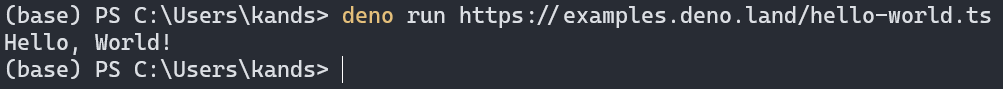
\includegraphics[scale=0.48]{pics/beginner-hello-world-p01.png}
    \caption{代码执行效果}
    \label{fig:beginner:hello-world:p01}
\end{figure}

\cls

\backmatter

\pagestyle{plain}
\setcounter{page}{1}
\pagenumbering{Roman}

\chapter*{Postscript | 后记}
\label{ch:postscript}
\addcontentsline{toc}{chapter}{Postscript | 后记}
这是后记
\cls

\listoffigures
\label{ch:figures}
\addcontentsline{toc}{chapter}{Figures | 图片清单}
\cls

\end{document}